%versi 3 (22-07-2020)
\chapter{Analisis}
\label{chap:analisis}

Pada bab ini akan dijelaskan analisis aplikasi WSDC 2017 Bali saat ini dan aplikasi WSDC yang akan dibangun. Analisis yang akan dibahas meliputi analisis {\it use case}, analisis kebutuhan sistem, dan analisis pembangunan aplikasi Android menggunakan Ionic.

\section{Analisis Sistem Kini}
\label{sec:analisisSistemKini}
Aplikasi WSDC 2017 Bali digunakan untuk menunjang keberlangsungan acara WSDC 2017 yang diselenggarakan di Bali, Indonesia. Aplikasi WSDC 2017 Bali dapat diunduh untuk sistem operasi {\it android} melalui URL \url{https://play.google.com/store/apps/details?id=org.wsdc2017indonesia.app&hl=en&gl=US}. Aplikasi ini dibangun dan dikembangkan oleh PT DNArtworks Komunikasi Visual yang rilis di Play Store pada tanggal 30 Juli 2017, dengan versi terakhir adalah versi 1.1.2 yang rilis pada 1 Agustus 2017. Selain rilis pada perangkat berbasis sistem operasi Android, aplikasi WSDC 2017 Bali juga sempat rilis untuk perangkat berbasis sistem operasi IOS. Namun, pada saat ini aplikasi WSDC 2017 Bali di perangkat berbasis sitem operasi IOS sudah diturunkan dari toko aplikasi App Store pada perangkat berbasis sitem operasi IOS. Untuk dapat mengakses aplikasi WSDC 2017 Bali, tidak diperlukan login. Pengguna dapat langsung membuka aplikasi dan akan ditampilkan halaman utama dari aplikasi WSDC 2017 Bali. Pada halaman utama pengguna dapat melihat berita-berita terkait acara WSDC 2017 Bali dan tombol {\it read more} yang apabila ditekan akan mengarahkan pengguna untuk mengunduh berita terkait acara WSDC 2017 Bali dengan format pdf. Aplikasi WSDC 2017 Bali dapat digunakan untuk melihat berita acara, pengumuman, jadwal peserta, lokasi acara, hasil pengundian, info, serta pengumuman pemenang dari acara WSDC 2017 Bali (Gambar~\ref{fig:useCaseDiagram}).

Aplikasi WSDC 2017 Bali dibangun menggunakan {\it framework} Ionic versi 3, dan Angular versi 4.1.3. Lalu untuk membangun aplikasi WSDC 2017 Bali agar dapat berjalan secara {\it native}, digunakanlah Cordova. Dengan digunakannya Cordova dan Ionic Framework, maka memungkinkan aplikasi WSDC 2017 Bali menggunakan teknologi HTML, dan CSS. Penggunaan Cordova juga memungkinkan aplikasi WSDC 2017 Bali kompatibel dengan perangkat berbasis Android dan IOS, tanpa perlu mengimplementasikannya kembali ke dalam bahasa masing-masing platform.

\begin{figure}[H]
		\centering
	    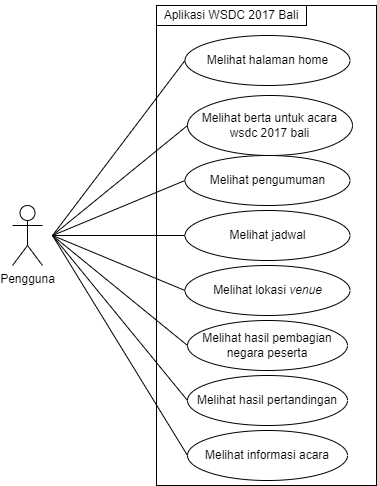
\includegraphics[scale=0.4]{Gambar/useCaseDiagram.png}
	    \caption{Diagram {\it Use Case} Aplikasi WSDC 2017 Bali}
	    \label{fig:useCaseDiagram}
\end{figure}

Terdapat fitur-fitur yang ada pada aplikasi WSDC 2017 Bali. Fitur-fitur tersebut adalah sebagai berikut :
\begin{enumerate}
	\item Halaman Utama
	\item Pemberitahuan
	\item Jadwal 
	\item {\it Venues}
	\item {\it Draw}
	\item Hasil
	\item Info
\end{enumerate}

\section{Analisis Sistem Usulan}
\label{sec:analisisSistemUsulan}